\documentclass{beamer}
\usetheme{default}
\usepackage{chemformula}

\title{Post-Christmas Update}
\author{Ben Goldmann}
\date{\today}

\usepackage{caption}
\captionsetup[figure]{labelformat=empty}
\captionsetup[table]{labelformat=empty}

\begin{document}

\begin{frame}
\titlepage
\end{frame}

\begin{frame}
\frametitle{Initial vs Refitted}

\begin{figure}
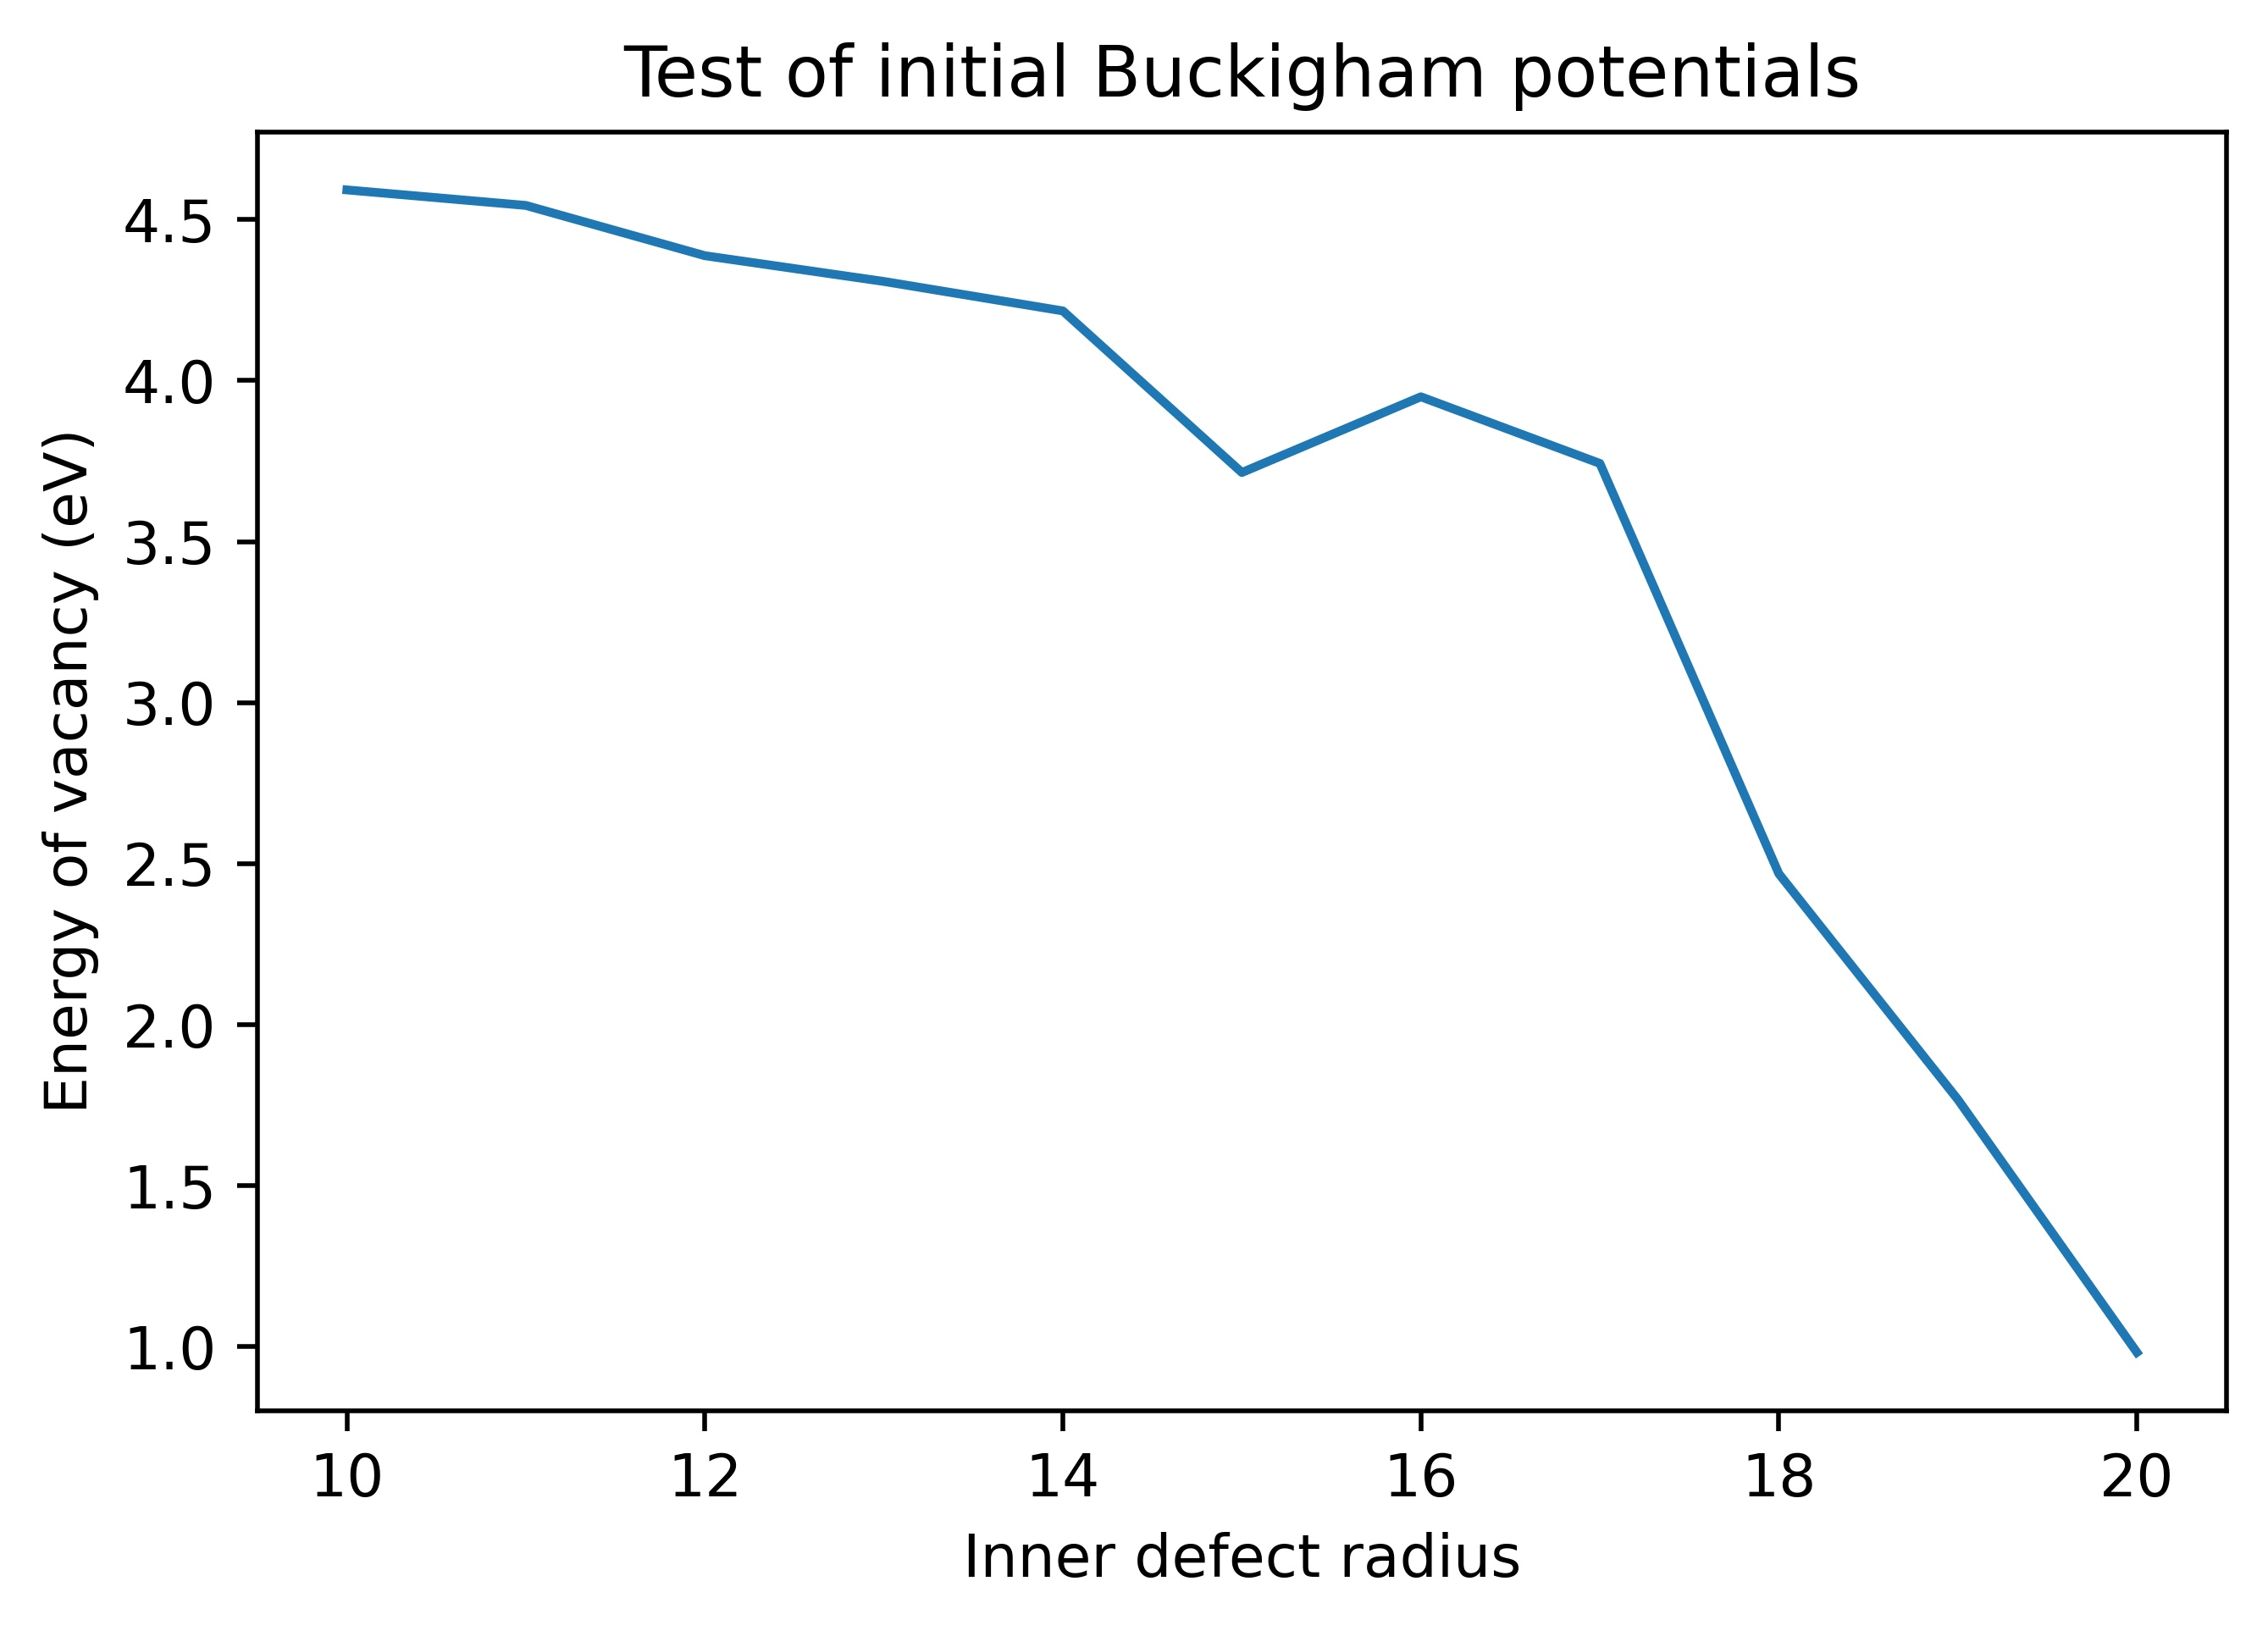
\includegraphics[width=0.5\textwidth]{/home/ben/Documents/gulp_calcs/0_summary/initial_test.jpg}%
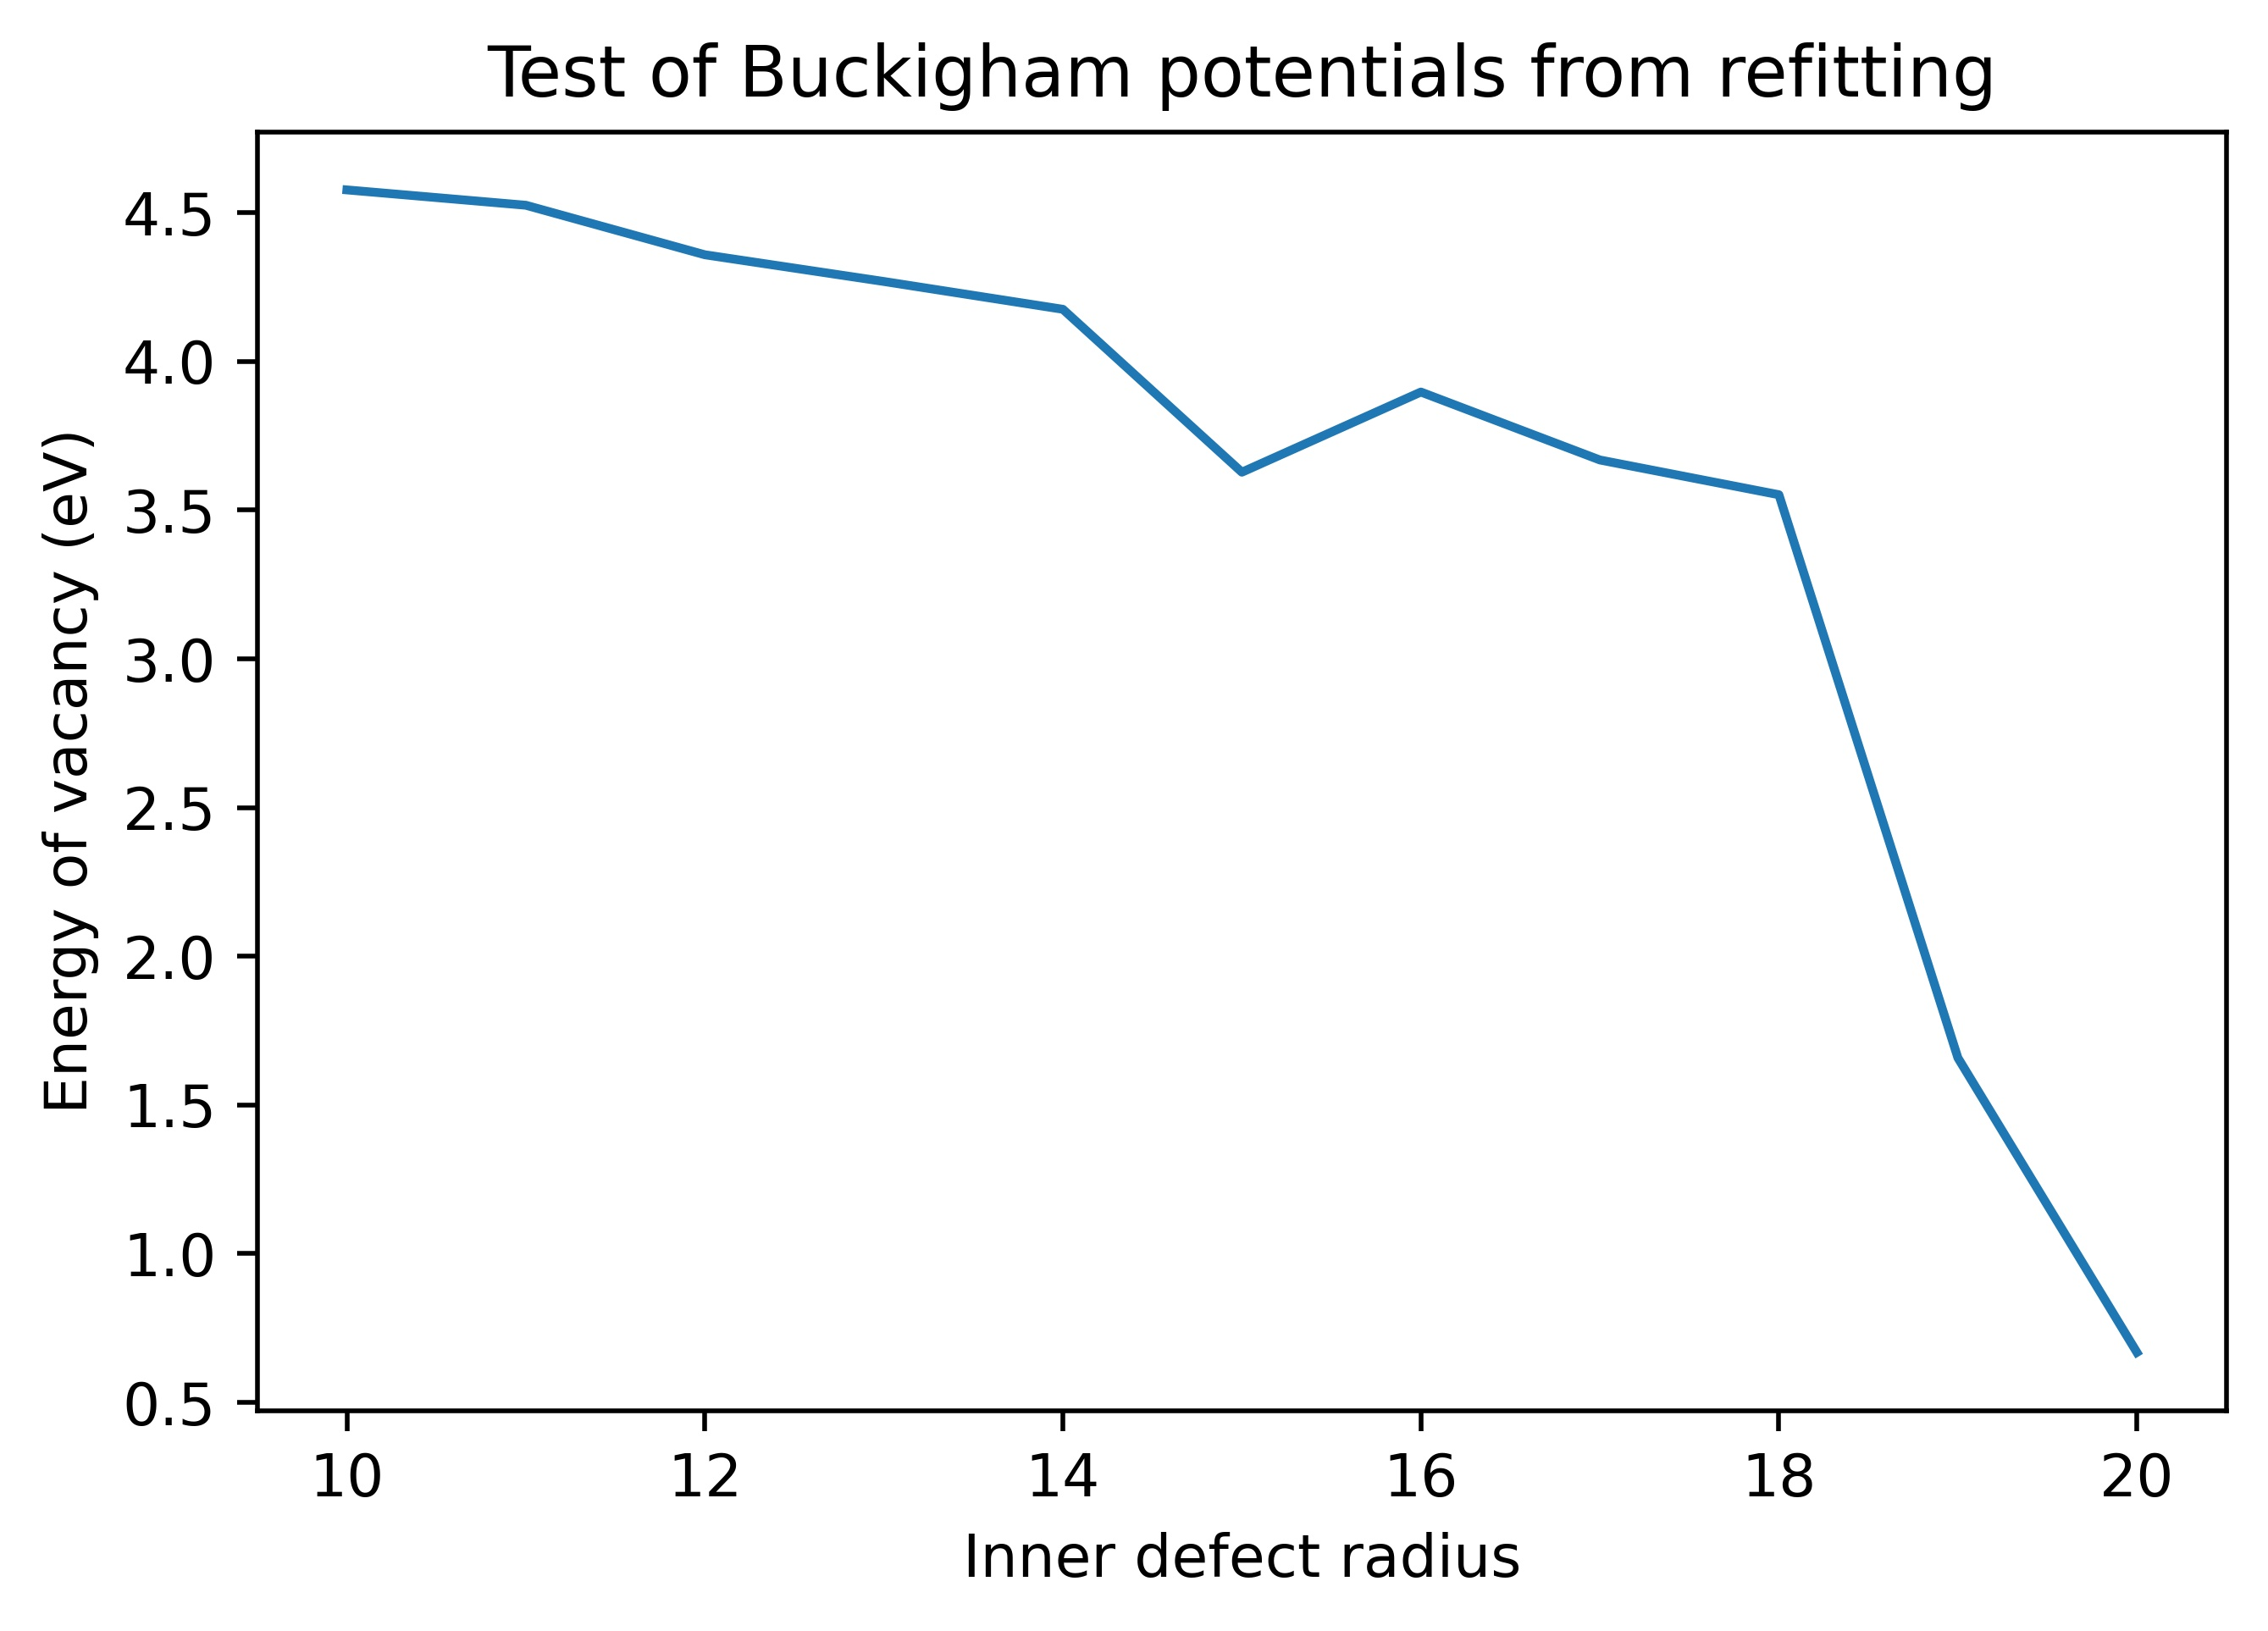
\includegraphics[width=0.5\textwidth]{/home/ben/Documents/gulp_calcs/0_summary/refitted_test.jpg}
\end{figure}

\begin{table}[h!]
  \begin{center}
    \caption{Buckingham potentials}
    \begin{tabular}{c|c|c}
      \hline
      Na-O & 1226.84 0.307 0 & 1225.11 0.307 0 \\
      Na-Cl & 2314.70 0.290 0 & 2292.53 0.290 0 \\
    \end{tabular}
  \end{center}
\end{table}

\end{frame}

\begin{frame}
\frametitle{Literature search}

\begin{figure}[ht]
  \begin{minipage}{0.45\linewidth}
    \centering
      \includegraphics[width=\textwidth]{/home/ben/Pictures/Deng2016.png}
      \caption{Deng at al. (2016)}
  \end{minipage}
  \hspace{0.5cm}
  \begin{minipage}{0.45\linewidth}
    \centering
    \includegraphics[width=\textwidth]{/home/ben/Pictures/Khandy2020.png}
    \caption{Khandy et al. (2020)}
  \end{minipage}
\end{figure}

\end{frame}

\begin{frame}
\frametitle{Data used and potentials calculated}

\begin{figure}
  \begin{minipage}{0.505\linewidth}
    \centering
      \begin{enumerate}
        \item Deng et al. (2016)
        \begin{itemize}
          \item Bulk modulus: 36.4 GPa
          \item Shear modulus: 24.6 GPa
          \item Na-O: 1042.96 0.310 0 \\ (vs 1226.84 0.307 0)
          \item Na-Cl:  1591.38 0.288 0 \\ (vs 2314.70 0.290 0)
        \end{itemize}
        \bigskip
        \item Khandy et al. (2020)
        \begin{itemize}
          \item Bulk Modulus: 33.45 GPa
          \item Shear modulus: 26.87 GPa
          \item Na-O: 588.38 0.338 0 \\ (vs 1226.84 0.307 0)
          \item Na-Cl: 1170.41 0.315 0 \\ (vs 2314.70 0.290 0)
        \end{itemize}
      \end{enumerate}
  \end{minipage}
  \hspace{0.5cm}
  \begin{minipage}{0.4\linewidth}
    \centering
    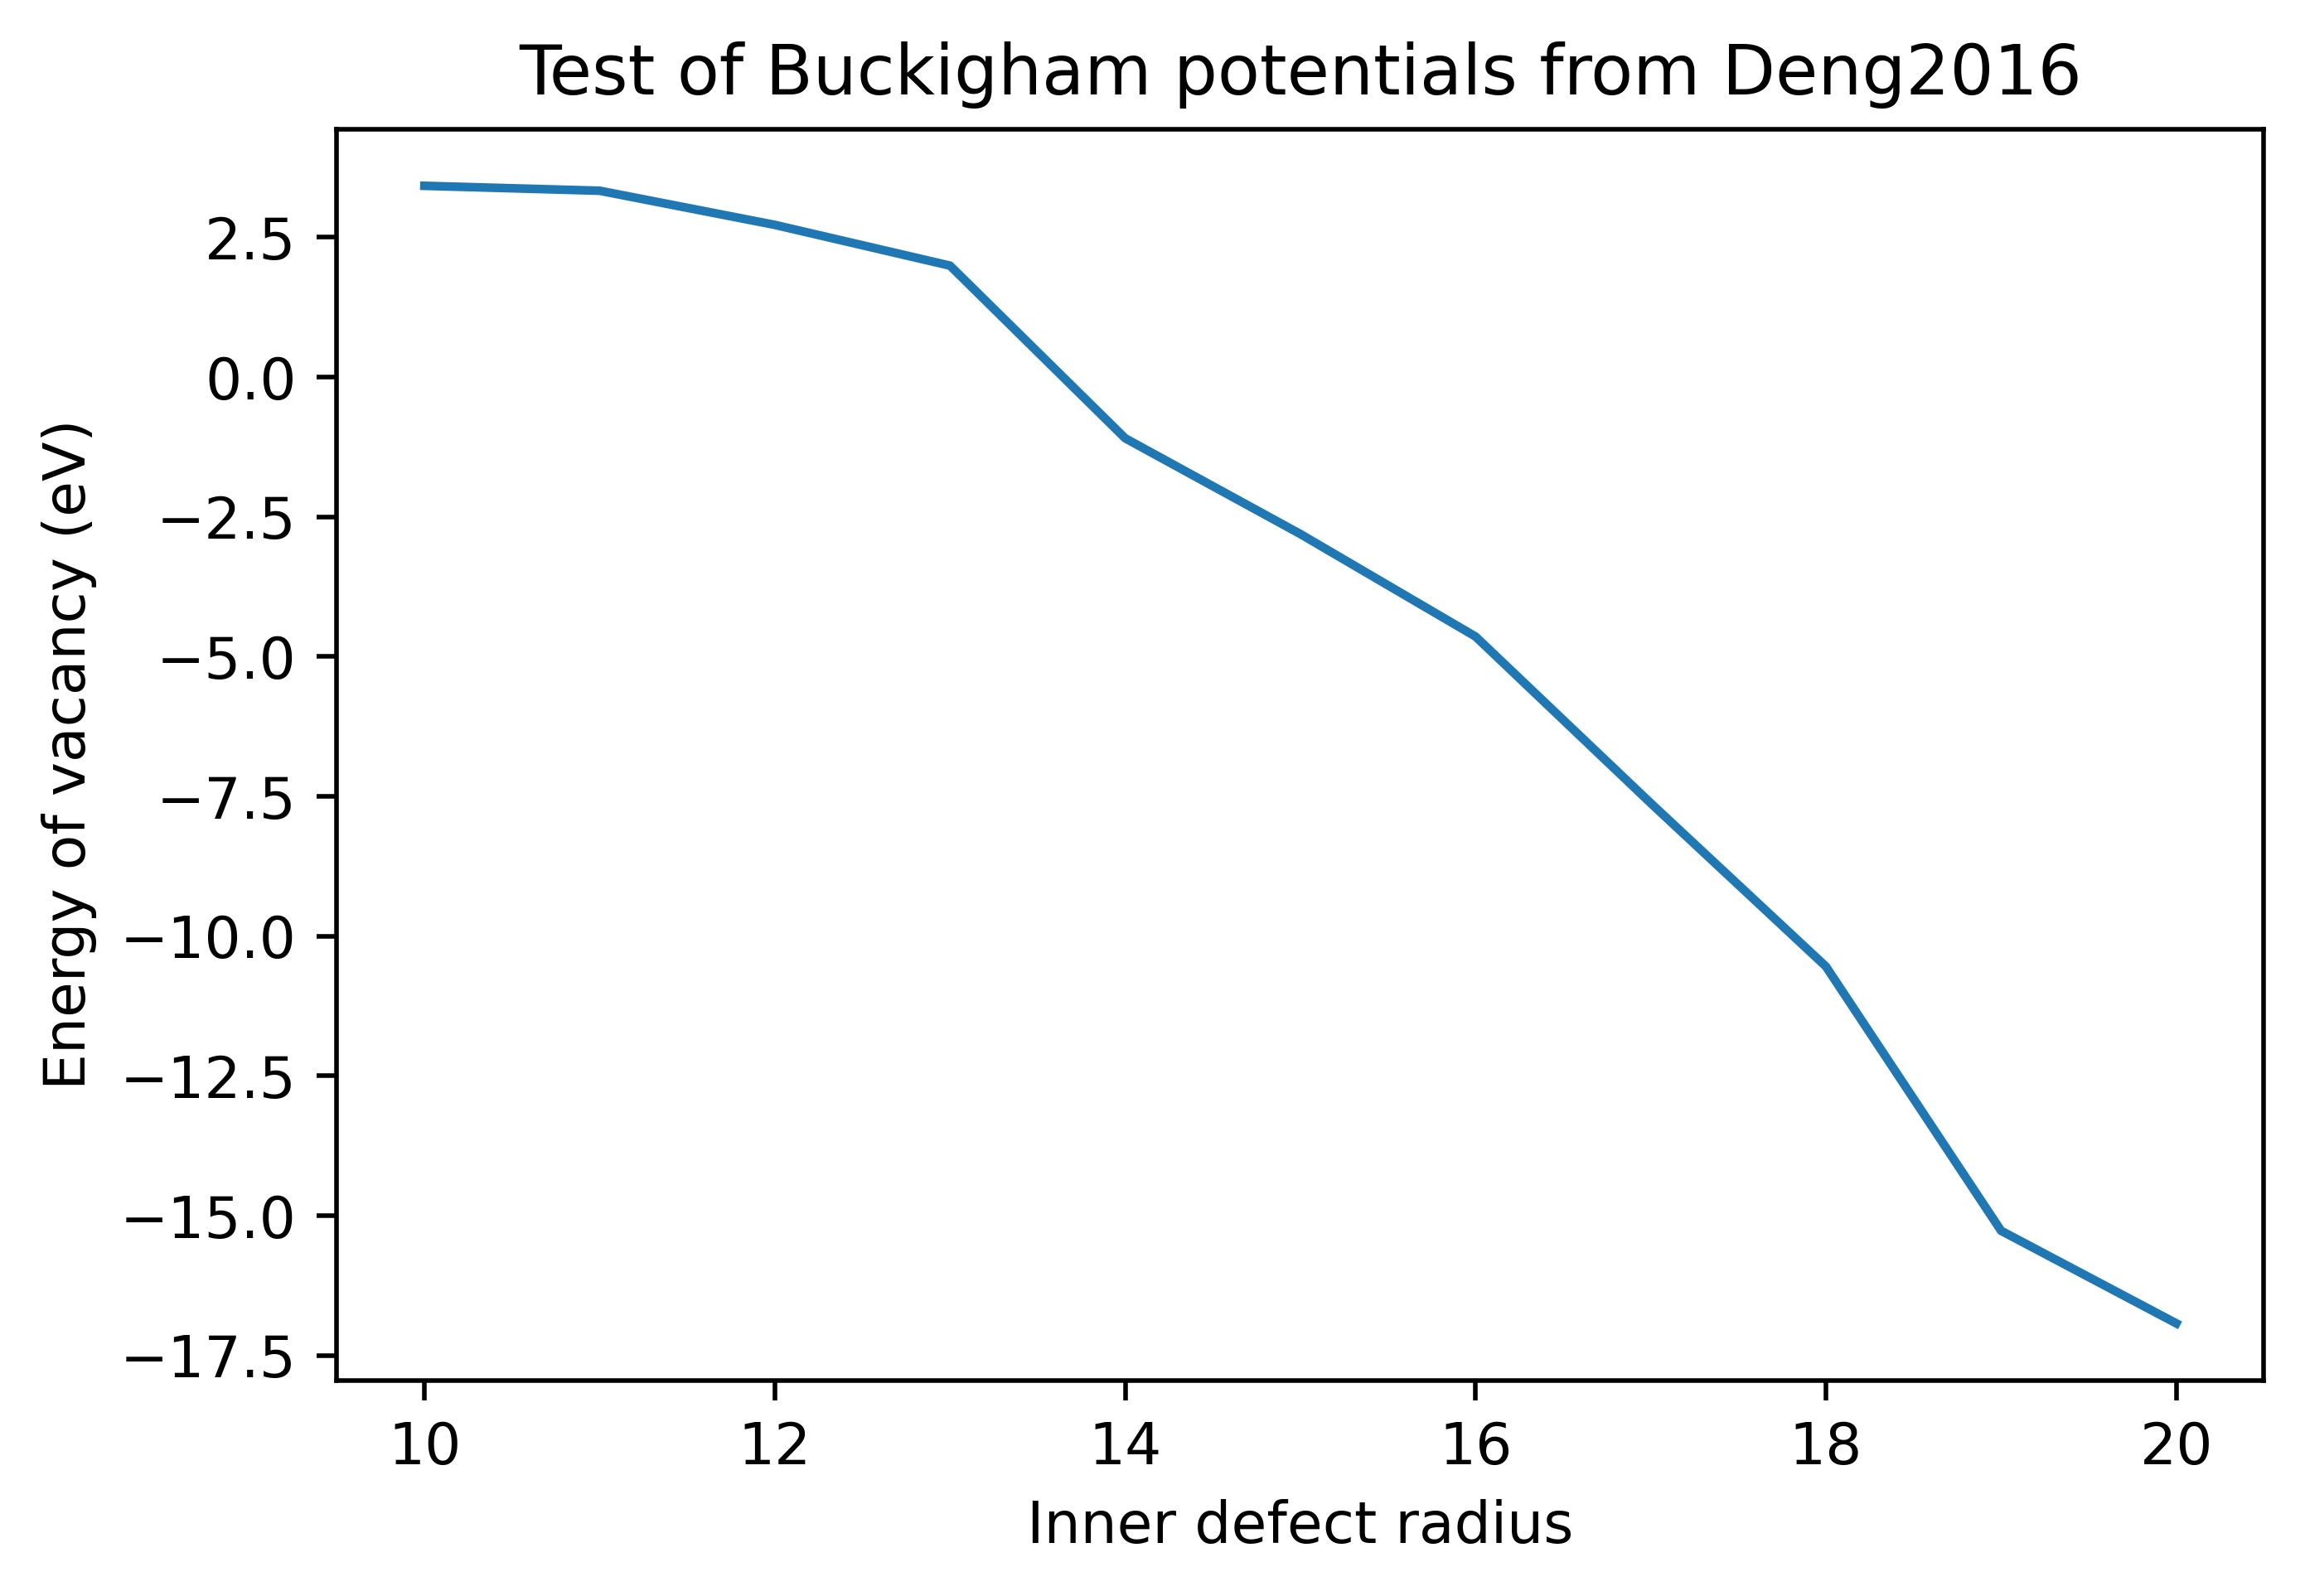
\includegraphics[width=\textwidth]{/home/ben/Documents/gulp_calcs/0_summary/deng_test.jpg}
    \caption{Deng2020}
    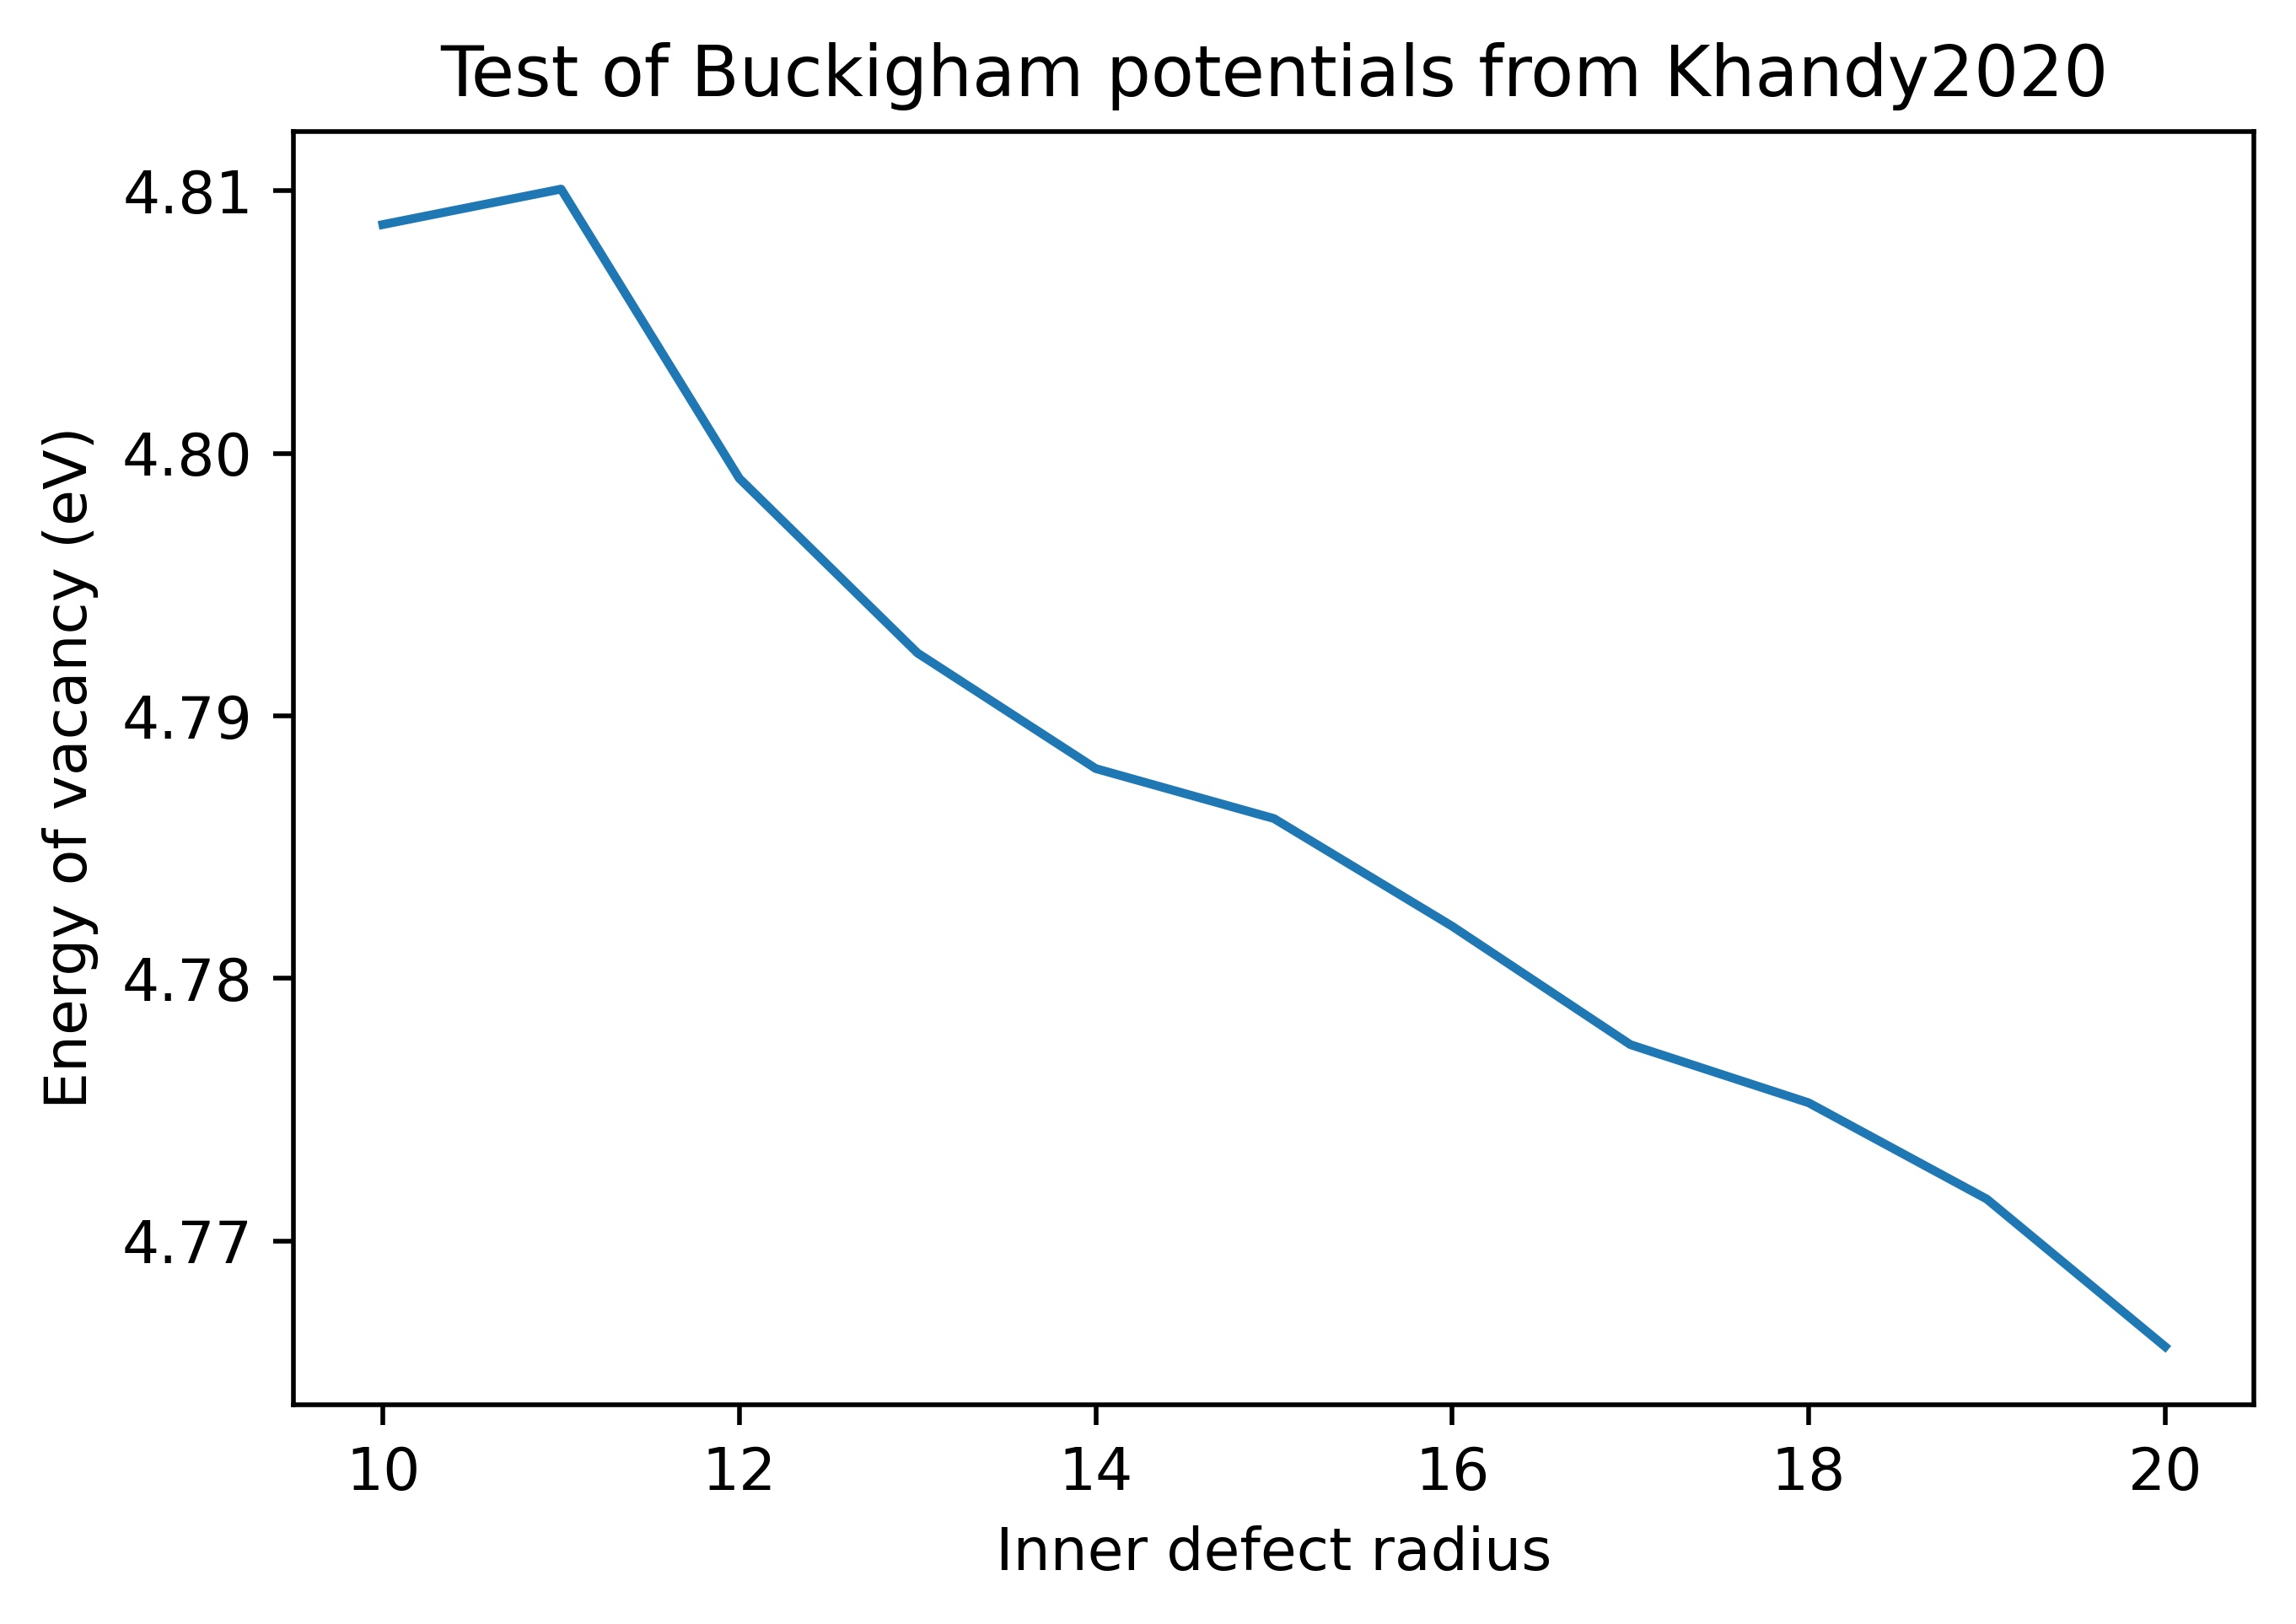
\includegraphics[width=\textwidth]{/home/ben/Documents/gulp_calcs/0_summary/khandy_test.jpg}
    \caption{Khandy2020}
  \end{minipage}
\end{figure}

\end{frame}

\begin{frame}
\frametitle{Comparison of Initial and Khandy}

\begin{figure}
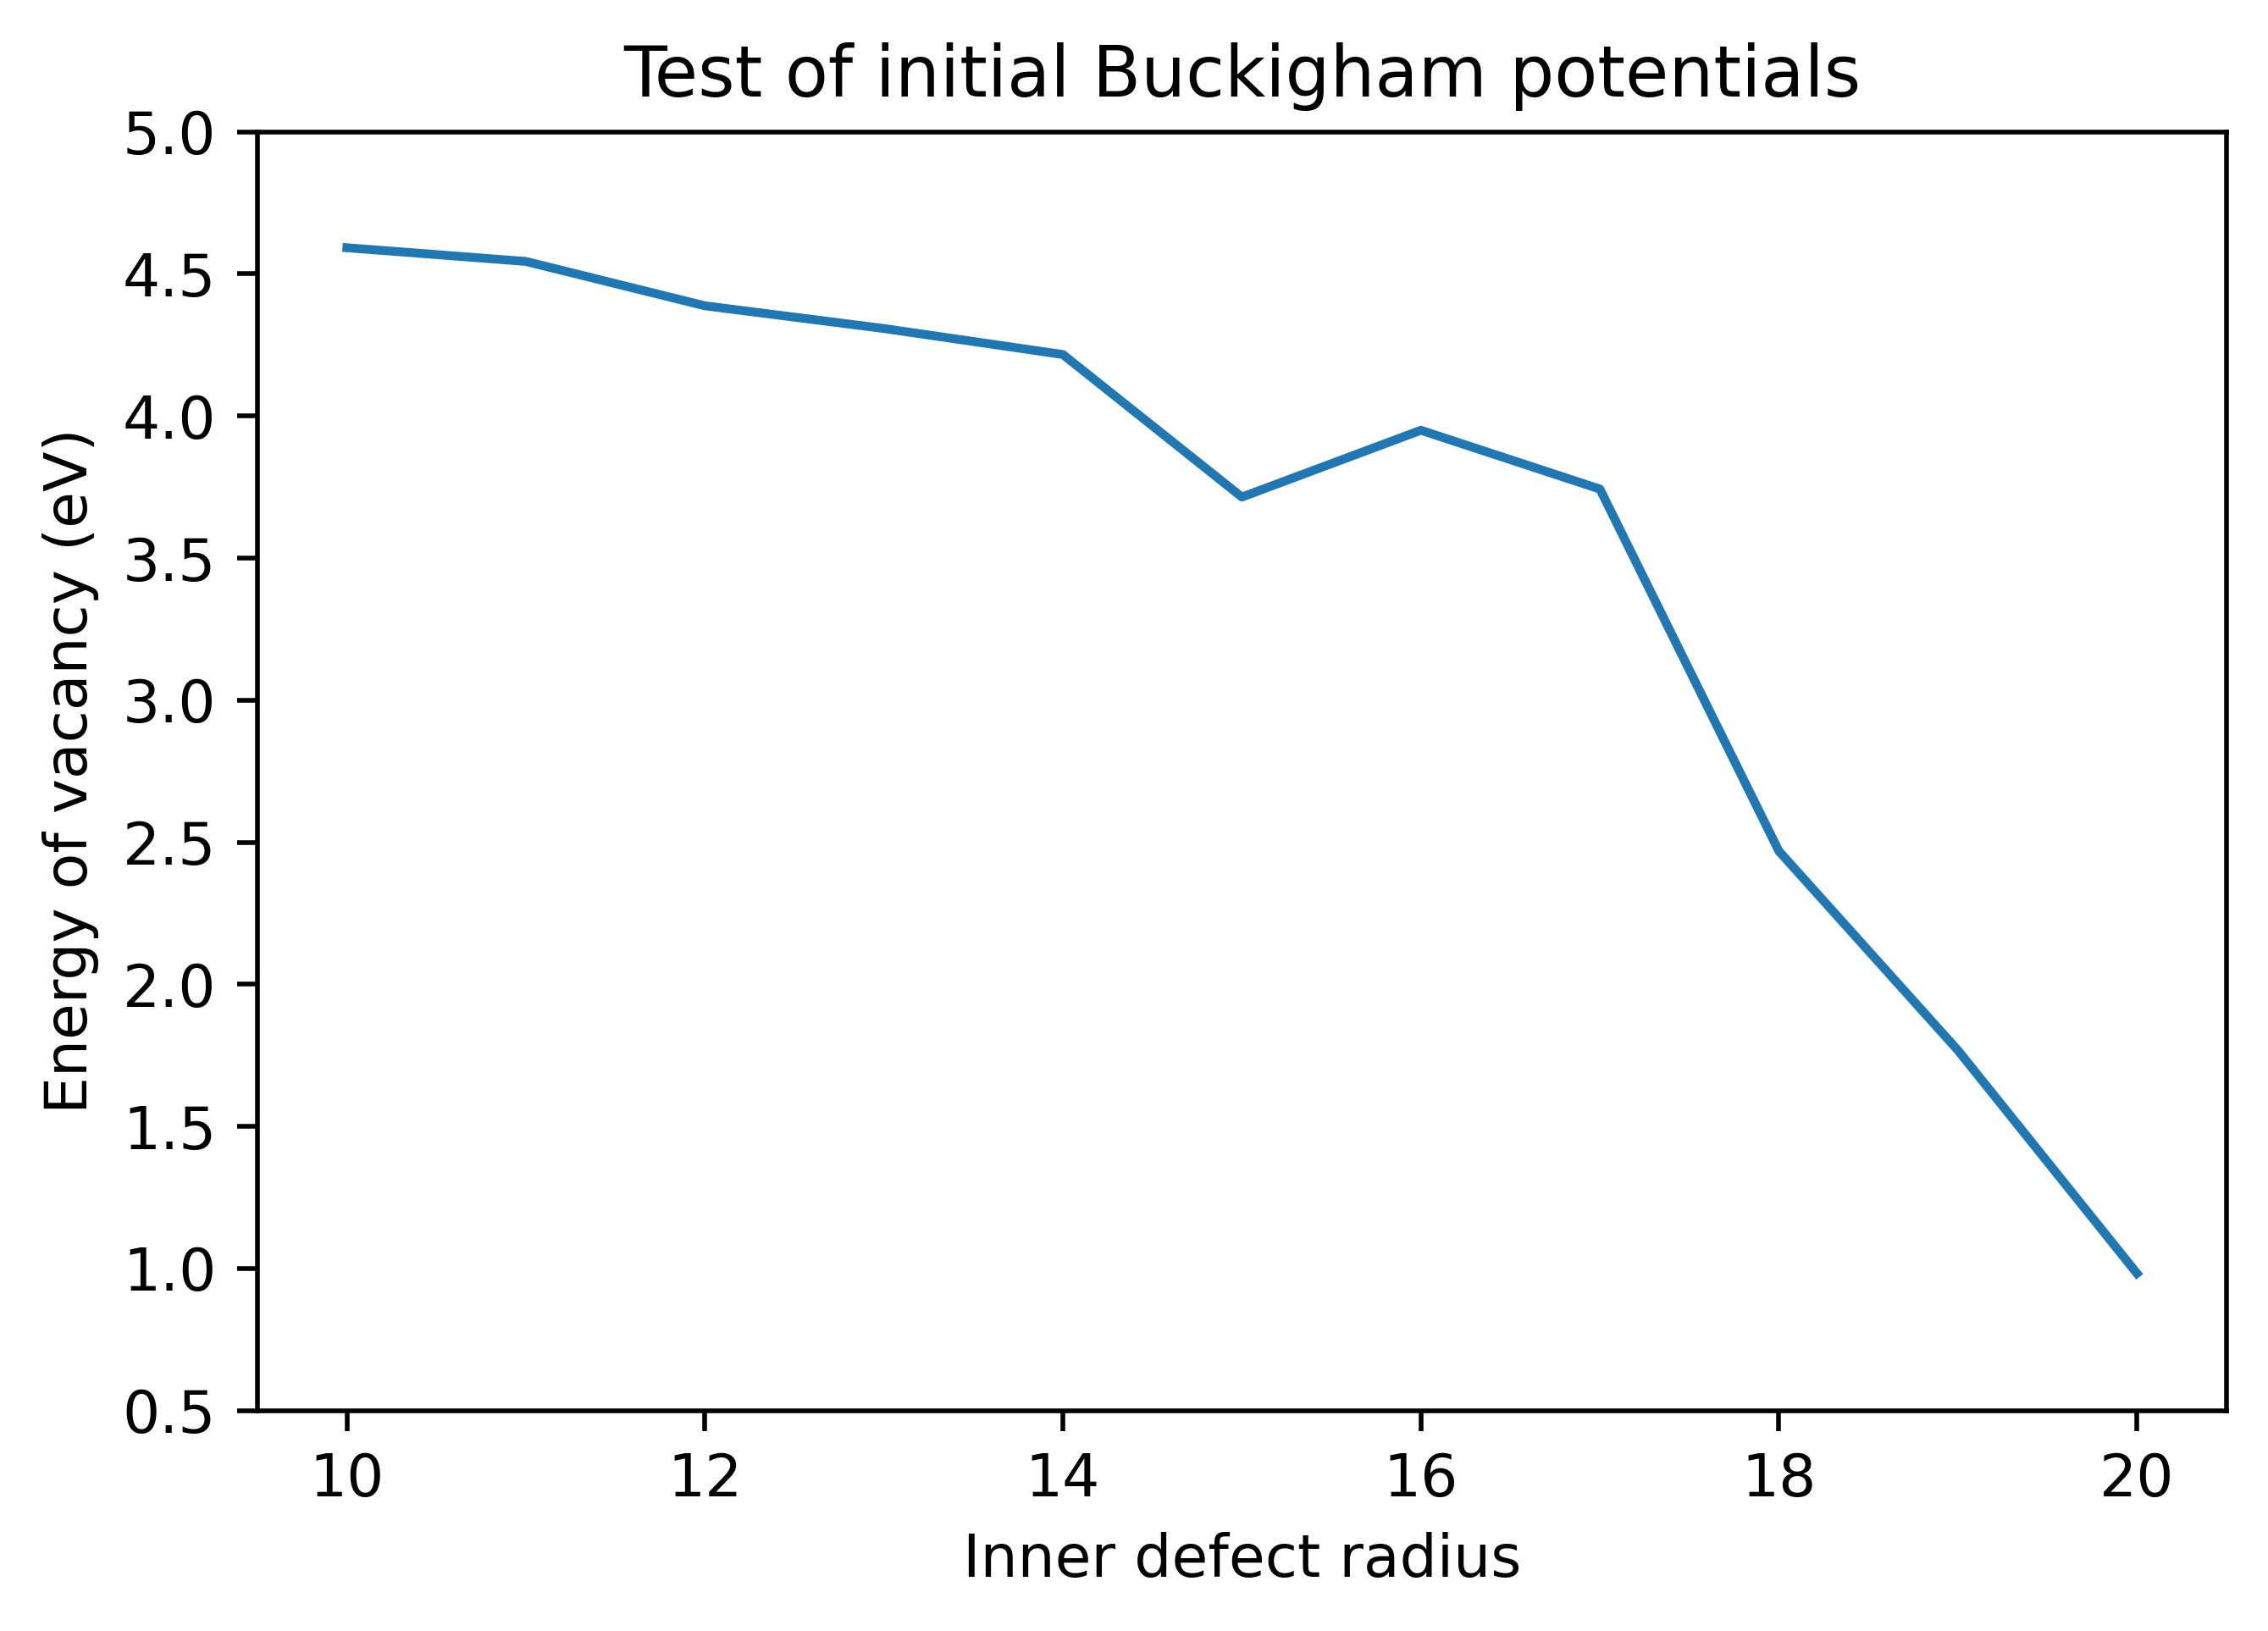
\includegraphics[width=0.5\textwidth]{/home/ben/Documents/gulp_calcs/0_summary/initial_test_scaled.jpg}%
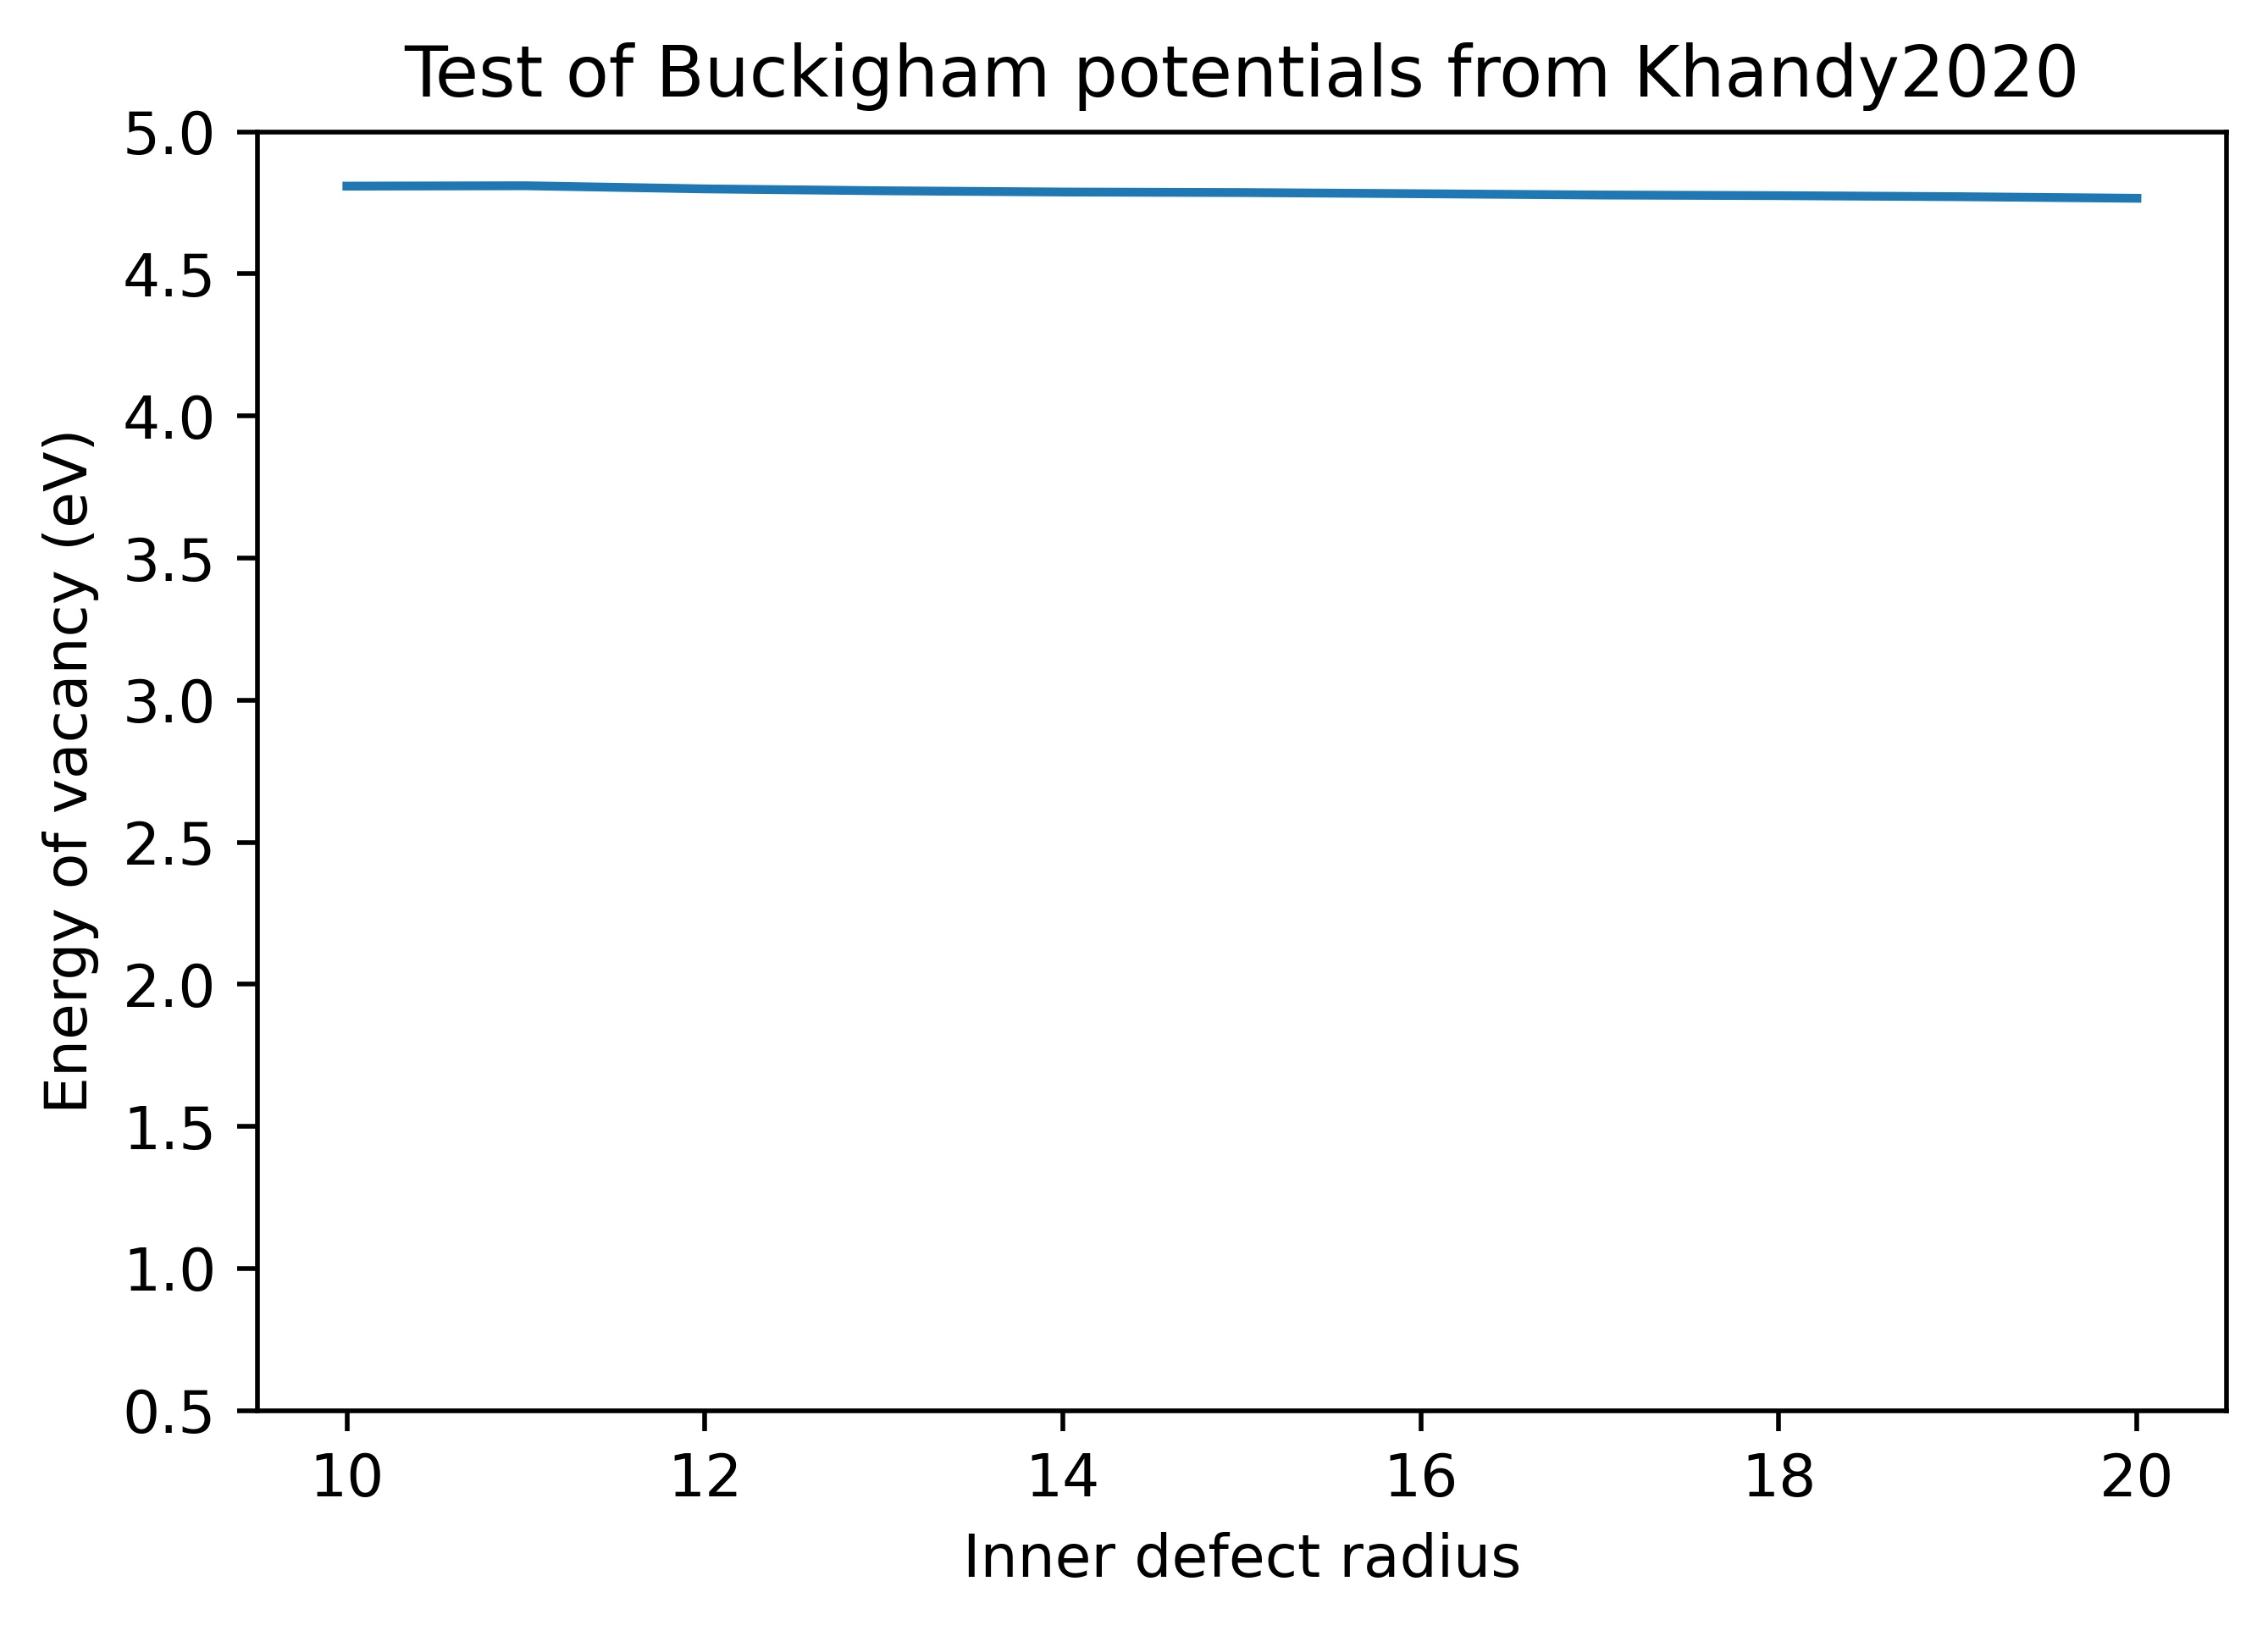
\includegraphics[width=0.5\textwidth]{/home/ben/Documents/gulp_calcs/0_summary/khandy_test_scaled.jpg}
\end{figure}

\end{frame}

\begin{frame}
\frametitle{Comparison of Initial and Khandy 2}

\begin{figure}
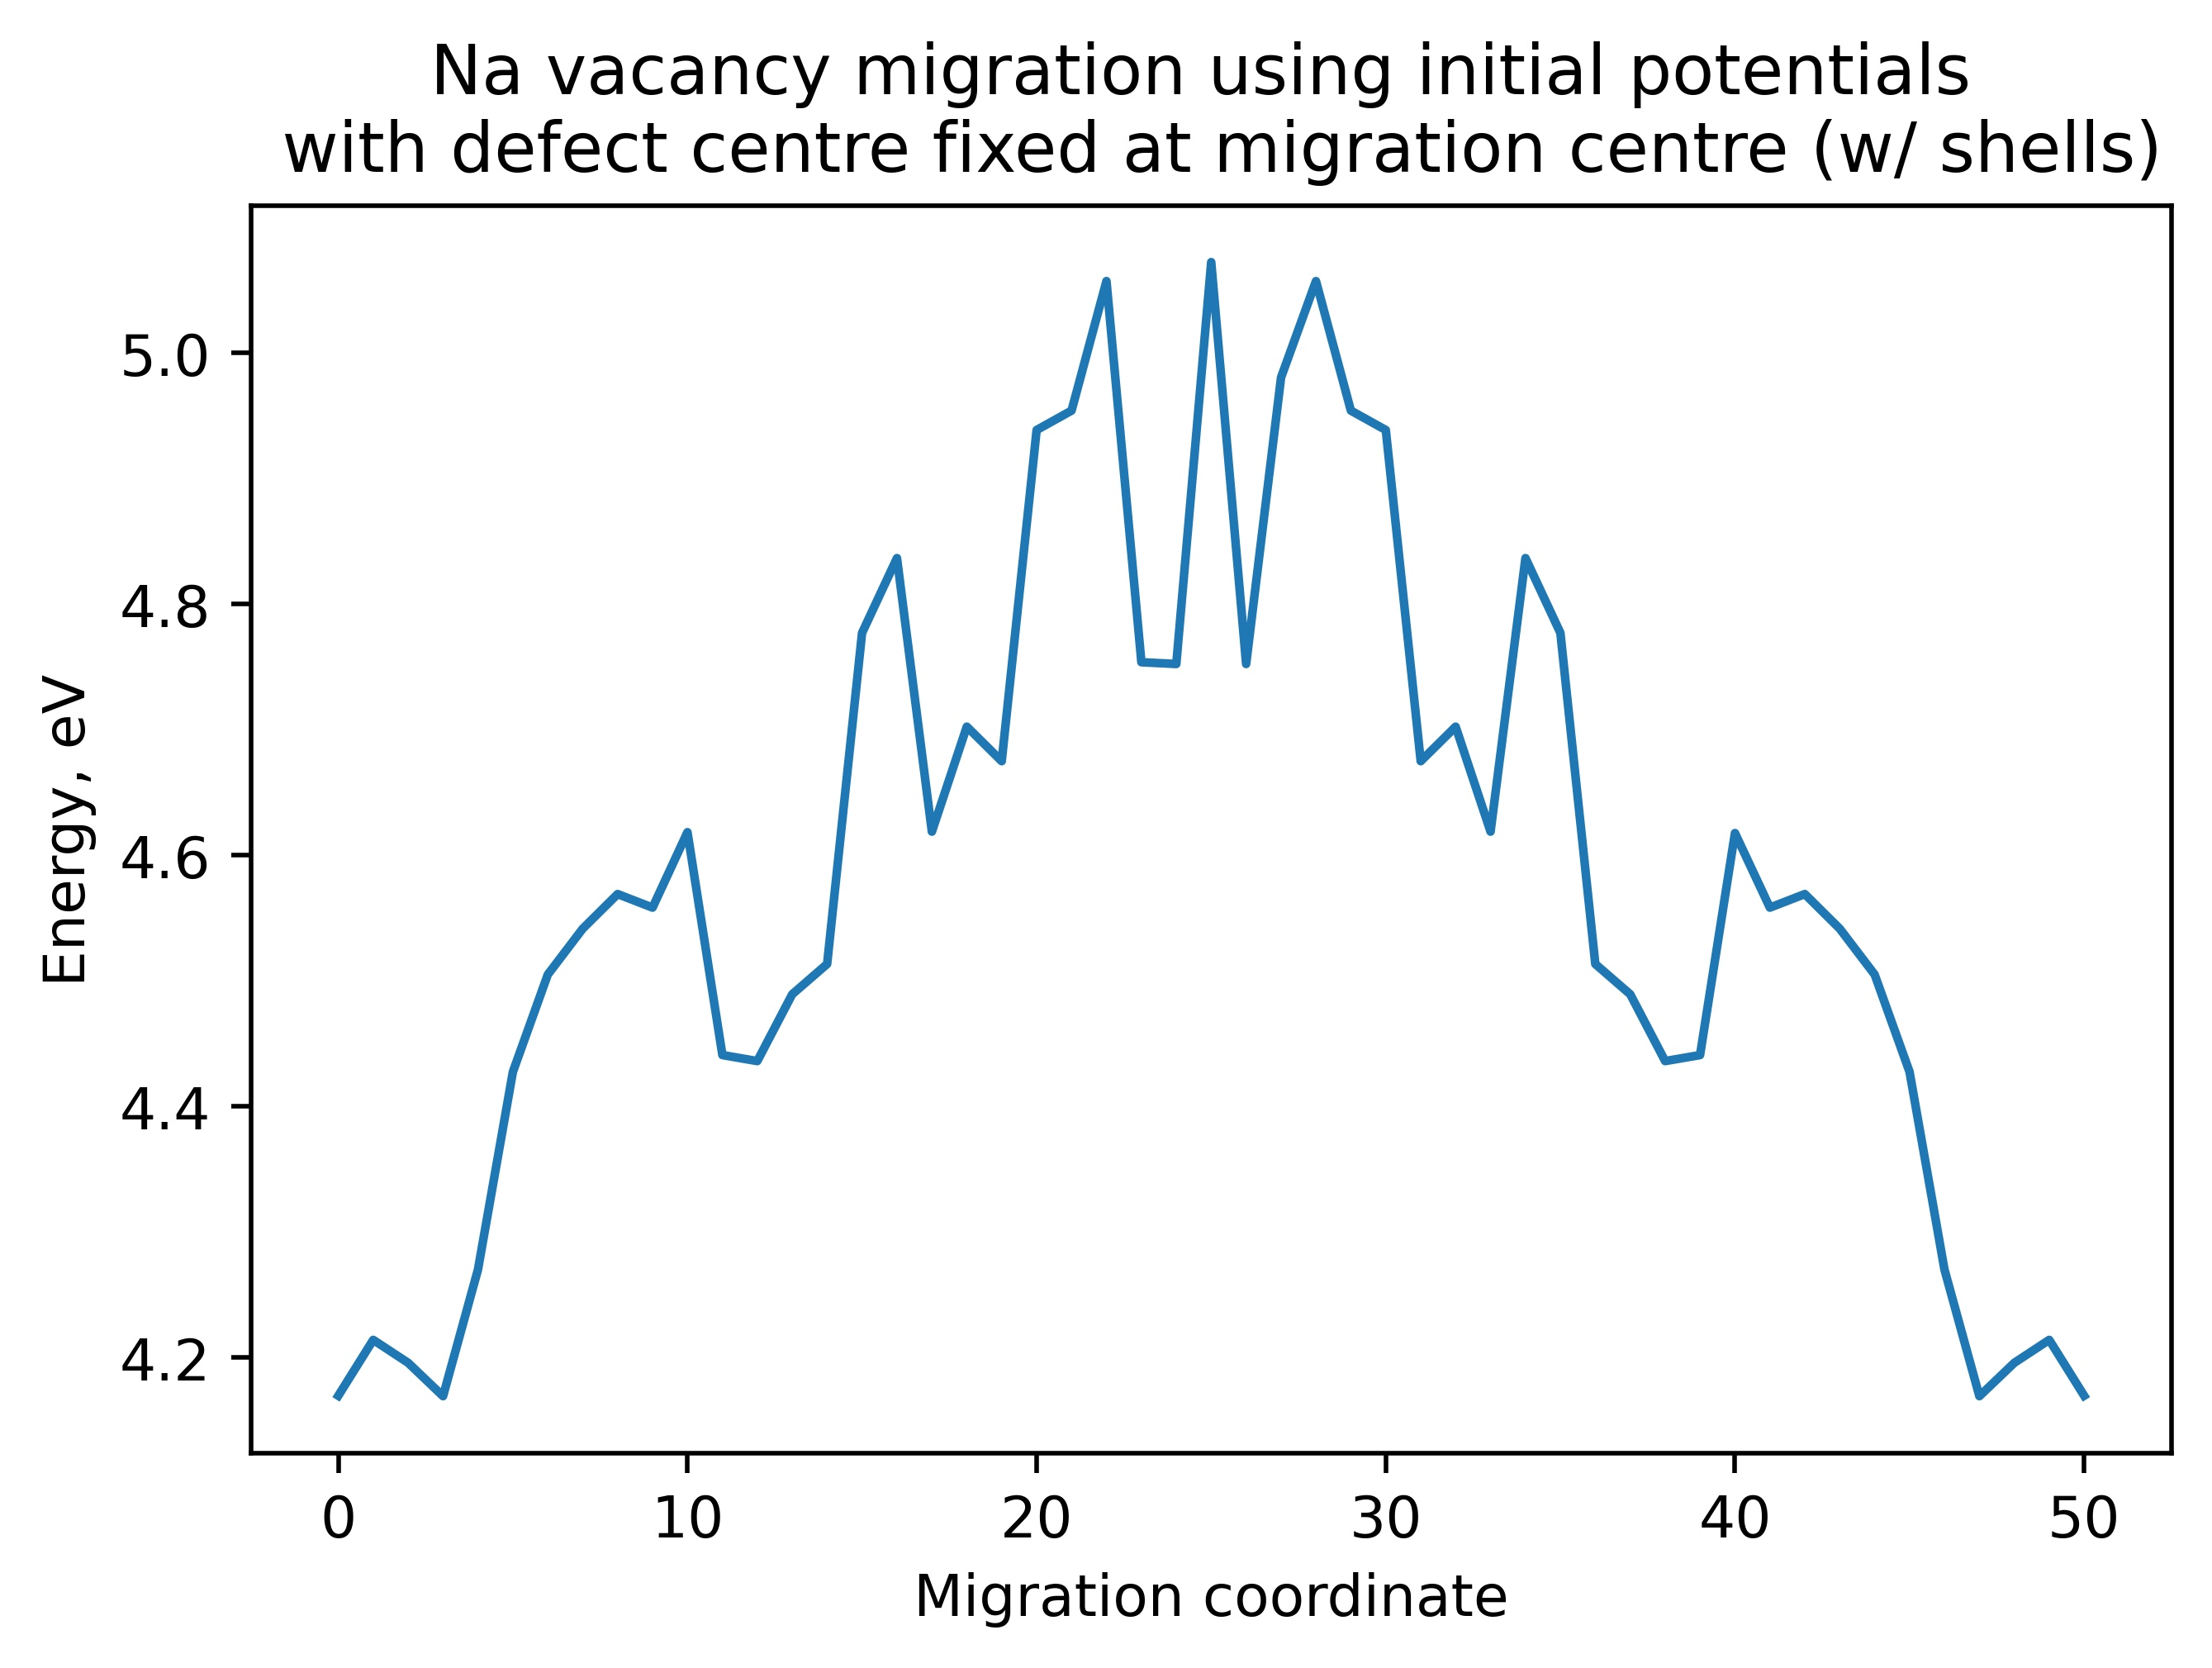
\includegraphics[width=0.5\textwidth]{/home/ben/Documents/gulp_calcs/0_summary/plot_na3ocl_fixcent_shel.jpg}%
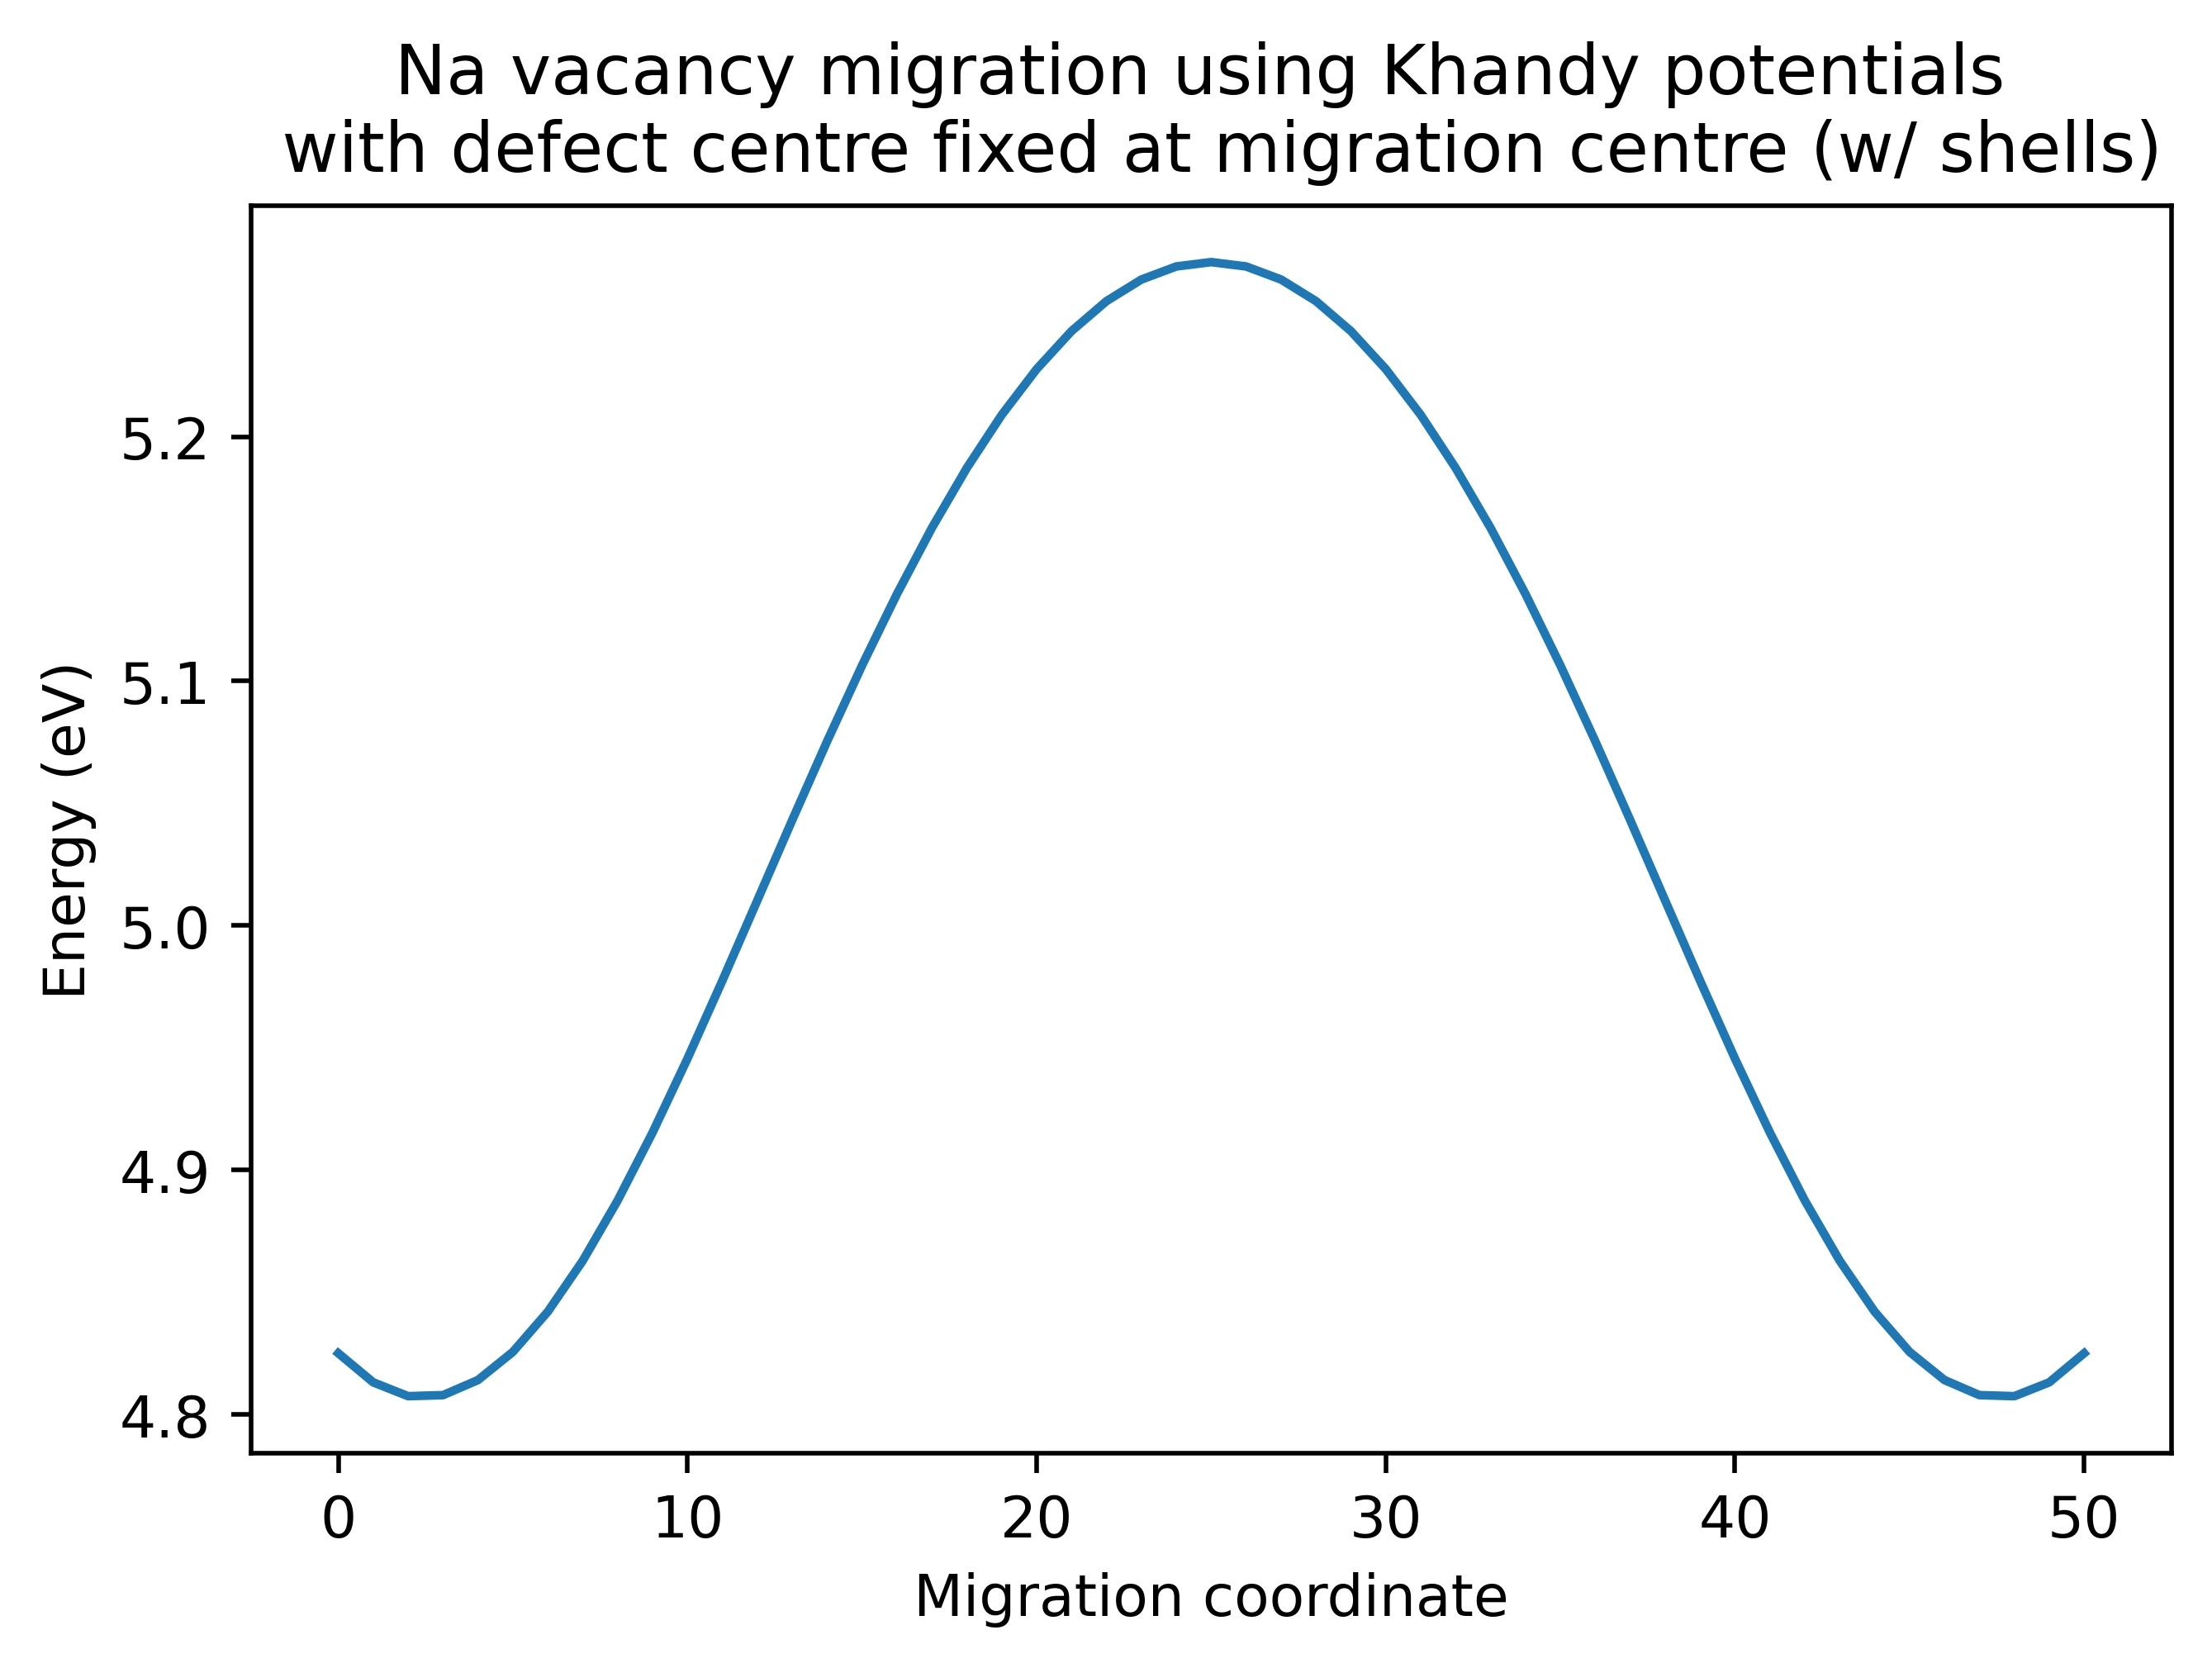
\includegraphics[width=0.5\textwidth]{/home/ben/Documents/gulp_calcs/0_summary/khandy_migration_fixcent.jpg}
\end{figure}

\end{frame}

\begin{frame}
\frametitle{Calculations using Khandy potentials}

\input{/home/ben/Documents/gulp_calcs/0_summary/output_na3ocl_khandy.txt}

\end{frame}

\end{document}